\documentclass[10pt,a4paper]{article}
\usepackage{graphicx} % Required for inserting images
\usepackage[margin=0.62in]{geometry}
\usepackage{amsmath,amssymb,amsthm,mathtools}
\usepackage{enumitem}
\usepackage{microtype}
\usepackage{tikz}
\usepackage{quantikz}
\usepackage{url}
\usepackage{booktabs}
\usepackage{pgfplots}
\pgfplotsset{compat=1.18}
\usetikzlibrary{positioning,arrows.meta,fit}
\setlength{\parindent}{0pt}
\setlength{\parskip}{1pt}

% figure style: data are inline, so the file compiles without image files
\definecolor{cblue}{HTML}{2A78D6}
\definecolor{corange}{HTML}{EB6834}
\definecolor{caqua}{HTML}{1BAF7A}
\definecolor{cgray}{HTML}{8A8F98}
\definecolor{cpurple}{HTML}{8E5CC9}
\pgfplotsset{
  every axis/.append style={font=\scriptsize, grid=major, grid style={gray!20},
    legend style={font=\tiny, draw=none, fill=white, fill opacity=0.85, text opacity=1},
    tick label style={font=\tiny}, label style={font=\scriptsize}, title style={font=\scriptsize}},
}

\title{Qiskit 2026 Track 1}
\author{Team: Three Qiskiteers}
\date{November 2026}

\begin{document}
{\centering\large\bfseries Qiskit 2026 Track 1 --- Three Qiskiteers\par}
\vspace{2pt}

\section{Exhaustive Search and Classification of Valid Passwords}

The elliptic-curve background used here (isogenies, kernels, torsion
subgroups, endomorphism rings, and supersingular curves) was studied
using Andrew Sutherland's MIT 18.783 lecture notes [6]. The
quantum-algorithmic background used below (Grover search, quantum
walks, and query complexity) was studied using Ronald de Wolf's
lecture notes [5]. The curve family and canonical bit conventions
below are the assignment's prescribed ones.

Let
\[
\mathbb F=\mathbb F_{1019}(i),\qquad i^2=-1,
\]
and let the initial curve parameter be
\[
A_0=977+297i.
\]
For a current parameter \(A_k\), define the two possible transitions by
\[
r_{0,1}=\frac{-A_k\pm\sqrt{A_k^2-4}}{2},
\]
where the roots are ordered according to
\[
\operatorname{key}(u+vi)=u+1019v,
\qquad 0\leq u,v<1019.
\]
The transition corresponding to bit \(b\in\{0,1\}\) is
\[
\boxed{
A_{k+1}=T_b(A_k)
=\operatorname{canonical}(2-4r_b^2),
}
\]
where the canonical representative is the one of \(z\) and \(-z\)
having the smaller key.

For a 12-bit string
\[
w=b_1b_2\cdots b_{12},
\]
iterate these transitions to obtain
\[
A_{12}=T_{b_{12}}\circ\cdots\circ T_{b_1}(A_0).
\]
The corresponding endpoint is accepted precisely when
\[
j(E_{A_{12}})
=\frac{256(A_{12}^2-3)^3}{A_{12}^2-4}
=797+921i
\quad\text{in }\mathbb F.
\]

\textbf{Exhaustive Enumeration.}
There are \(2^{12}=4096\) possible 12-bit strings. Evaluating the
transition rule for each string and testing its terminal
\(j\)-invariant gives exactly 37 valid passwords. These passwords
fall into three classes according to their final canonical
parameter. The full list of the 37 passwords is in
\texttt{results/part1\_L12.txt} of the repository.

\begin{table}[ht]
\centering
\small
\begin{tabular}{c c c}
\hline
\textbf{Final parameter \(A_{12}\)}
& \textbf{Number of passwords}
& \textbf{Terminal \(j\)-invariant}\\
\hline
\(3+10i\)       & 14 & \(797+921i\)\\
\(933+205i\)    & 9  & \(797+921i\)\\
\(561+411i\)    & 14 & \(797+921i\)\\
\hline
\textbf{Total} & \textbf{37} & \\
\hline
\end{tabular}
\caption{Classification of all valid 12-bit passwords.}
\end{table}

\textbf{Quantum completeness is a separate requirement.} The list above is a
finite-instance reference enumeration; classical enumeration alone is not the
quantum completeness certificate required by the problem rules. In the
unstructured phase-oracle model, finding all $k$ marked routes among $N$
possibilities has optimal query complexity $\Theta(\sqrt{Nk})$ [11], not
the $\Theta(\sqrt{N/k})$ cost for finding just one. For $N=4096$ and
$k=37$, the scale is $\sqrt{Nk}\approx389$ phase-oracle queries. A complete
submission must additionally specify how it handles unknown $k$, the case
$k=0$, and an overall failure probability $\varepsilon$; the classical list
above does not establish those points. Each phase-oracle query must be charged
for its compute--mark--uncompute implementation (24 one-step calls when
$L=12$).

\textbf{Our quantum run.} The one-step circuit is a 22-qubit permutation built
from the survey (255 spots, 510 roads walked once). Iterative amplitude
estimation on the phase oracle pins $k=37$ at confidence $\ge0.99$
(Fig.~\ref{fig:p1}, left); $k=0$ would give an interval at $0$ and the code
reports ``no route''. Grover search with 8 iterations per run then returns
all 37 routes, each confirmed by one classical walk. The run used 881{,}088
one-step queries, almost all of them in the high-confidence count
(Fig.~\ref{fig:p1}, right): at $N=4096$ the constants of the counting
dominate, while the scaling is $\sqrt{Nk}$.

\begin{figure}[ht]
\centering
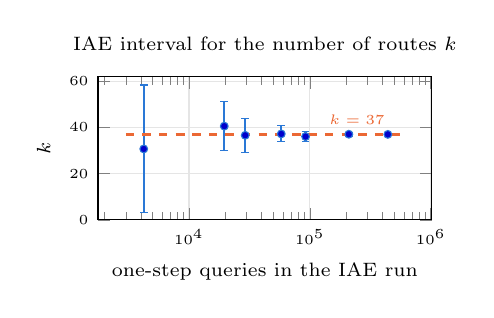
\begin{tikzpicture}
\begin{axis}[width=0.48\linewidth, height=3.4cm, xmode=log,
  xlabel={one-step queries in the IAE run}, ylabel={$k$},
  title={IAE interval for the number of routes $k$}, ymin=0, ymax=62]
\addplot+[cblue, only marks, mark=*, mark size=1.4pt,
  error bars/.cd, y dir=both, y explicit, error bar style={cblue, line width=0.8pt}]
  coordinates {(4224,30.738) +- (0,27.669) (19584,40.603) +- (0,10.582)
  (29184,36.640) +- (0,7.294) (57984,37.242) +- (0,3.474)
  (92160,36.100) +- (0,2.071) (210048,37.105) +- (0,0.914)
  (441600,37.038) +- (0,0.426)};
\addplot[corange, dashed, thick, domain=3000:600000] {37};
\node[corange, font=\tiny, anchor=south east] at (axis cs:500000,37) {$k=37$};
\end{axis}
\end{tikzpicture}\hfill
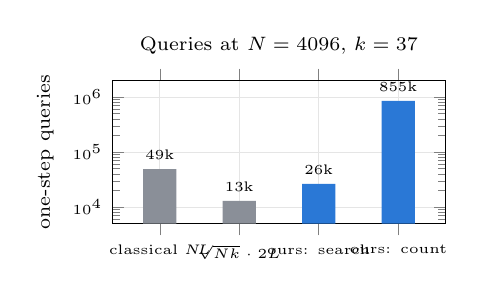
\begin{tikzpicture}
\begin{axis}[width=0.48\linewidth, height=3.4cm, ybar, bar width=12pt,
  ymode=log, log origin=infty, ymin=5000, ymax=2e6,
  xtick={1,2,3,4}, xmin=0.4, xmax=4.6,
  xticklabels={classical $N\!L$, $\sqrt{Nk}\cdot 2L$, ours: search, ours: count},
  x tick label style={font=\tiny, align=center, text width=1.5cm},
  ylabel={one-step queries}, title={Queries at $N=4096$, $k=37$},
  nodes near coords, nodes near coords style={font=\tiny},
  point meta=explicit symbolic]
\addplot[fill=cgray, draw=none, bar shift=0pt] coordinates {(1,49152) [49k] (2,13013) [13k]};
\addplot[fill=cblue, draw=none, bar shift=0pt] coordinates {(3,26304) [26k] (4,854784) [855k]};
\end{axis}
\end{tikzpicture}
\caption{Part I. Left: the counting interval narrows to $k=37$. Right: queries
of our run against the classical and optimal quantum scales.}
\label{fig:p1}
\end{figure}

\section{Part II: Quantum Search on the Supersingular Isogeny Graph}
\footnotesize

\subsection{Target set and its density}

Let \(V_p\) be the vertex set of the supersingular \(2\)-isogeny
graph over \(\mathbb F_{p^2}\), and define the target set
\[
T_p=\{j\in V_p:j\in\mathbb F_p\}.
\]
Writing \(j=u+vi\), with \(u,v\in\mathbb F_p\) and \(i^2=-1\),
the target condition is simply \(v=0\).

For \(p\equiv3\pmod4\), the Deuring--Eichler
\textbf{Class-Number Formula} gives
\[
|T_p|=
\begin{cases}
2h(-p),&p\equiv3\pmod8,\\
h(-p),&p\equiv7\pmod8,
\end{cases}
\]
where \(h(-p)\) is the class number of
\(\mathbb Q(\sqrt{-p})\) [3]. Moreover,
\[
|V_p|=\frac p{12}+O(1)=\Theta(p).
\]
By the Dirichlet class-number formula and Siegel's theorem,
\[
h(-p)=p^{1/2+o(1)}.
\]
Consequently, the proportion of target vertices is
\[
\boxed{\frac{|T_p|}{|V_p|}=p^{-1/2+o(1)}.}
\]

\subsection{From vertex density to route density}

A binary string \(x\in\{0,1\}^L\) specifies a
non-backtracking walk of length \(L\). Let \(A_L(x)\) denote
its terminal curve parameter and define
\[
f(x)=
\begin{cases}
1,&j(E_{A_L(x)})\in\mathbb F_p,\\
0,&\text{otherwise}.
\end{cases}
\]
Let \(q_L=\Pr_{x\leftarrow\{0,1\}^L}[f(x)=1]\).

The supersingular $2$-isogeny graph is $3$-regular, and the
Ramanujan property of supersingular isogeny graphs follows from
the corresponding Hecke-operator eigenvalue bounds; see the survey
of Florit Zacar\'ias [7] and Pizer's Hecke-operator construction [9].
We use the non-backtracking random-walk estimate of Lubetzky--Peres
[8, Theorem 3.5 and equation (3.13)]. A closely matching statement
specialized to supersingular isogeny graphs is also given by Mula,
Murru, and Pintore [10, Theorem 2.14]: a non-backtracking walk of
length at least $(1+\epsilon)\log_\ell p$ has endpoint distribution
within $\widetilde O(p^{-\epsilon/2})$ of uniform. For the standard supersingular $2$-isogeny graph, connectedness is standard
[9]; non-bipartiteness follows from the degree-two self-isogeny $[1+i]$ of
the supersingular $j=1728$ curve when $p\equiv3\pmod4$ (so the graph has a
loop, with loops retained). We also assume the two bits sample the two
non-backtracking outgoing edges uniformly. Write $n_p=|V_p|$ and let
$\widetilde\mu_L$ be the distribution of the final directed edge.
For a fixed starting directed edge, their estimate gives, for
$d=3$ and $N_E=3n_p$ directed edges,
\[
\left\|\frac{\widetilde\mu_L}{\pi_E}-1\right\|_{L^2(\pi_E)}^2
\le 2N_E2^{-L}(8L^2+1),
\]
where $\pi_E$ is uniform on directed edges. By
Cauchy--Schwarz,
\[
d_{\rm TV}(\widetilde\mu_L,\pi_E)
\le O\!\left(\sqrt{n_p}\,2^{-L/2}L\right).
\]
Projecting a directed edge to its endpoint cannot increase total
variation distance, and the endpoint projection of $\pi_E$ is
uniform on vertices. Since $n_p=\Theta(p)$, taking
\[
L=\left\lceil3\log_2p\right\rceil
\]
gives $d_{\rm TV}(\mu_L,U_p)=O(p^{-1}\log p)=\widetilde O(p^{-1})$.
If the component is bipartite, the walk alternates between the
two directed-edge classes; one must instead use the parity-conditioned
stationary law and the target density in the reachable class.
Under the stated non-bipartite hypothesis, total variation bounds
probability discrepancy for every event, so
\[
q_L=\frac{|T_p|}{|V_p|}+O(p^{-1}\log p)
     =\boxed{p^{-1/2+o(1)}}.
\]
Thus a uniformly random length-$L$ route is marked with
probability $q_L$.

\subsection{Grover search: construction of the marking oracle}

There are \(N=2^L\) candidate routes and, writing \(k\) for
the number of marked routes, \(q_L=k/N\). Grover's algorithm
searches this route space in superposition. The phase-oracle and amplitude-amplification viewpoint is standard; see de Wolf's quantum-computing notes [5].

Starting with
\[
|s\rangle=\frac1{\sqrt N}\sum_{x\in\{0,1\}^L}|x\rangle,
\]
a reversible computation evaluates the \(L\) isogeny steps
controlled by \(x\), computes the terminal invariant
\[
j(E_{A_L(x)})=u(x)+v(x)i,
\]
and sets a flag equal to \([v(x)=0]\). A phase flip is applied
when this flag is \(1\). The computation is then uncomputed,
so the route register is left unchanged except for its phase.
The resulting phase oracle is
\[
\boxed{O_f|x\rangle=(-1)^{f(x)}|x\rangle.}
\]
In particular, this is not an assumed free oracle: it is
implemented by \(L\) forward isogeny-step computations,
the reversible target test, and \(L\) inverse steps.
Thus one marking operation costs \(2L\) one-step calls,
apart from the finite-field arithmetic for the test.

The Grover diffusion operator \(D=2|s\rangle\langle s|-I\)
is then alternated with \(O_f\). If
\[
\theta=\arcsin\sqrt{q_L},
\]
after \(t\) iterations the success probability is
\[
P_G(t)=\sin^2((2t+1)\theta).
\]
Choosing \(t=\Theta(q_L^{-1/2})\) gives constant success
probability. Hence
\[
t=O(p^{1/4+o(1)}),
\qquad
\boxed{Q_{\rm step}=p^{1/4+o(1)}.}
\]
This is the quantum upper bound, including the
\(L=\Theta(\log p)\) cost of each marking operation.

\subsection{Classical comparison}

Independent random route evaluations succeed with probability
\(q_L\). The expected number of evaluations before the first
success is \(1/q_L\). Therefore
\[
Q_{\rm classical}
=\Theta(q_L^{-1})
=p^{1/2+o(1)}
\]
complete-route evaluations, or
\[
\boxed{Q_{\rm classical,step}=p^{1/2+o(1)}}
\]
one-step calls. Grover's algorithm gives a quadratic
improvement in the inverse success probability.

\subsection{Lower bound in the black-box model}

To state a rigorous lower bound, consider the
\textbf{Unstructured Quantum Search Model}. Its input is an
unknown Boolean function
\[
f:X\longrightarrow\{0,1\},\qquad
X=\{0,1\}^L,\quad |X|=N,
\]
promised to have exactly \(k\) marked inputs. The algorithm
accesses the marked set only through the oracle
\[
O_f|x,z\rangle=|x,z\oplus f(x)\rangle
\]
and must output a marked \(x\).

The \textbf{Zalka Optimality Theorem} [1] and the BBBV lower bound [4] state that any quantum
algorithm achieving constant success probability requires
\[
\Omega\!\left(\sqrt{\frac Nk}\right)
=\Omega(q_L^{-1/2})
\]
oracle queries. Since \(q_L=p^{-1/2+o(1)}\), this becomes
\[
\boxed{Q_{\rm oracle}=\Omega(p^{1/4-o(1)}).}
\]
Together with Grover's upper bound, this establishes the
\(p^{1/4+o(1)}\) search exponent in the unstructured
black-box model.

The model qualification is essential. The actual isogeny
transition is explicit algebraic finite-field arithmetic.
An algorithm with direct access to that structure may exploit
relations between routes or vertices that an arbitrary
Boolean oracle does not reveal. Thus Zalka's theorem is a
lower bound for the black-box abstraction, not an
unconditional lower bound for every algorithm solving the
explicit arithmetic problem. If each route-oracle query is
required to be implemented serially using \(2L\) step calls,
the corresponding step-call lower bound in that restricted
model is \(\Omega(Lp^{1/4-o(1)})\).

{\footnotesize
\textbf{Related path-finding algorithms.} The standard $\ell$-\textsc{IsogenyPath}
problem asks, given two supersingular curves, for any path between them;
$\ell$ fixes the degree of each edge, not the number of edges [12]. Page and
Wesolowski [13, Proposition 8.6] give a generic bidirectional algorithm with
expected time $\operatorname{poly}(\ell,\log p) p^{1/2}$, memory
$O(p^{1/2})$, and output path length $O(\log p)$. For fixed $\ell=2$, this is
$\widetilde O(\sqrt p)$. In the present setting one may choose a fixed
Clock-Tower target: $j=1728$ if $p\equiv7\pmod{12}$, or $j=0$ if
$p\equiv11\pmod{12}$. The algorithm is therefore a relevant classical
benchmark, but it uses walks from both endpoints and a collision search, so
it is explicitly forbidden by the assignment's no-backtracking/no-meet-in-
the-middle rule.

Delgado [14] gives an unconditional Las Vegas algorithm with expected time
and memory $p^{1/3}\exp(O(\sqrt{\log p\,\log\log p}))=p^{1/3+o(1)}$ for
\textsc{OneEnd}; known reductions extend this to EndRing and unrestricted
isogeny problems. This is not directly an unconditional fixed-$\ell$ path
algorithm. Transferring it to $\ell$-\textsc{IsogenyPath} through Wesolowski's
reduction [12] invokes GRH. Moreover, that reduction uses a path parameter
$e=\lceil(\log p)^c/\log\ell\rceil$, giving a polylogarithmic length bound,
not automatically a $\Theta(\log p)$ bound. These results reinforce that the
black-box lower bound here is not a lower bound for every algorithm using the
explicit arithmetic structure.\par
}

\subsection{Experimental exponent fitting}

For each tested prime \(p\), let \(M_p\) be the number of
random routes sampled and \(S_p\) the number ending in
\(\mathbb F_p\). The empirical density is
\[
\widehat q_p=\frac{S_p}{M_p}.
\]
To test the predicted power law, fit
\[
\widehat q_p\approx Cp^{-\alpha},
\qquad
\log\widehat q_p=\log C-\alpha\log p.
\]
For 65 primes $p\equiv3\pmod4$ from $2^{10}$ to $2^{26}$, with $4\cdot10^5$
random routes of length $L=2\lceil\log_2p\rceil$ each, the reported regression is
\[
\boxed{\widehat q_p\approx8.7\,p^{-0.523},}
\qquad
\boxed{\widehat\alpha=0.523\pm0.040,}
\]
and the exact spot fractions (40 primes up to $2^{20}$) give
$\widehat\alpha=0.560\pm0.081$ (two standard errors).
This is consistent with the theoretical exponent
\(\alpha=\tfrac12\); finite-sample variation and class-number
fluctuations mean that the fitted exponent need not equal
\(\tfrac12\) exactly. The experiment is supporting evidence,
not a proof of the asymptotic estimate.

\textbf{Demonstration.} On the campus $p=5923$, $A_0=66+1530i$, $L=12$, a
fraction $q=1/39.8\le1/32$ of the routes ends on the Clock Tower. The
25-qubit circuit (transpiled to $\{cx,rz,sx,x\}$, one Grover iteration:
24 queries, $3.40\cdot10^6$ CX, depth $1.11\cdot10^7$) follows
$\sin^2((2t+1)\theta)$ to four decimals and reaches $0.981$ at $t=4$, where
classical walking with the same number of queries reaches $0.205$
(Fig.~\ref{fig:p2}, right). With $q$ unknown, BBHT needs on average 91 queries
and 7.9 classical checks, against 477 steps for classical random routes.

\begin{figure}[ht]
\centering
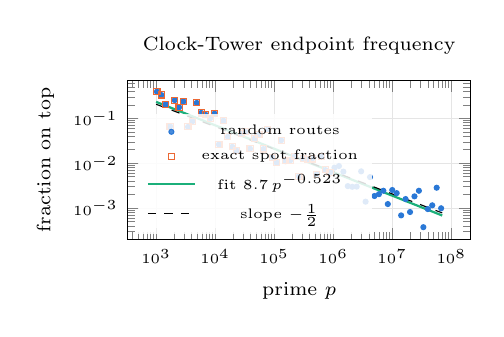
\begin{tikzpicture}
\begin{axis}[width=0.49\linewidth, height=3.6cm, xmode=log, ymode=log,
  xlabel={prime $p$}, ylabel={fraction on top},
  title={Clock-Tower endpoint frequency}, legend pos=south west, ymin=2e-4, ymax=0.7]
\addplot[cblue, only marks, mark=*, mark size=0.9pt] coordinates {
(1031,0.393470) (1223,0.332168) (1451,0.206083) (1723,0.066175) (2063,0.255248) (2447,0.176725) (2903,0.238303) (3463,0.064702) (4099,0.085947) (4871,0.221660) (5807,0.132830) (6899,0.119650) (8219,0.100453) (9743,0.127342) (11587,0.026270) (13799,0.088703) (16411,0.038730) (19507,0.023152) (23203,0.019015) (27583,0.046608) (32771,0.049340) (38971,0.021050) (46351,0.035153) (55127,0.043280) (65539,0.020665) (77951,0.056717) (92683,0.013760) (110251,0.010287) (131111,0.032575) (155887,0.011060) (185371,0.011465) (220447,0.014045) (262147,0.005150) (311747,0.012795) (370759,0.012230) (440903,0.012778) (524347,0.005667) (623531,0.014090) (741467,0.007010) (881779,0.006275) (1048583,0.007975) (1247063,0.008670) (1482919,0.006493) (1763491,0.003090) (2097211,0.002980) (2493979,0.003012) (2965847,0.006598) (3526987,0.001390) (4194319,0.004908) (4987903,0.001860) (5931763,0.002043) (7053971,0.002437) (8388619,0.001230) (9975803,0.002527) (11863343,0.002155) (14107963,0.000687) (16777259,0.001590) (19951627,0.000817) (23726579,0.001825) (28215851,0.002433) (33554467,0.000375) (39903203,0.000950) (47453183,0.001153) (56431751,0.002845) (67108879,0.000990)};
\addlegendentry{random routes}
\addplot[corange, only marks, mark=square, mark size=1.1pt] coordinates {
(1031,0.39535) (1223,0.33333) (1451,0.20661) (1723,0.06729) (2063,0.25581) (2447,0.17647) (2903,0.23967) (3463,0.06467) (4099,0.08683) (4871,0.22167) (5807,0.13223) (6899,0.12000) (8219,0.10073) (9743,0.12808) (11587,0.02658) (13799,0.08870) (16411,0.03924) (19507,0.02317) (23203,0.01948) (27583,0.04640) (32771,0.05016) (38971,0.02145) (46351,0.03538) (55127,0.04354) (65539,0.02081) (77951,0.05727) (92683,0.01368) (110251,0.01019) (131111,0.03222) (155887,0.01129) (185371,0.01150) (220447,0.01386) (262147,0.00502) (311747,0.01266) (370759,0.01213) (440903,0.01247) (524347,0.00553) (623531,0.01395) (741467,0.00720) (881779,0.00612)};
\addlegendentry{exact spot fraction}
\addplot[caqua, thick, domain=1000:7e7, samples=2] {8.660*x^(-0.523)};
\addlegendentry{fit $8.7\,p^{-0.523}$}
\addplot[black, dashed, domain=1000:7e7, samples=2] {6.538*x^(-0.5)};
\addlegendentry{slope $-\frac12$}
\end{axis}
\end{tikzpicture}\hfill
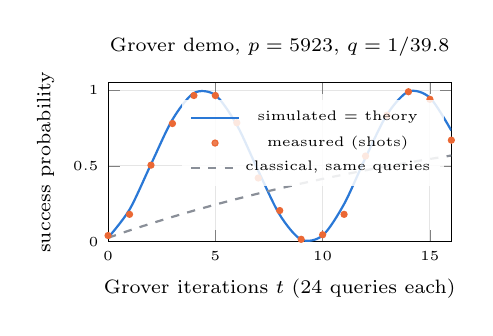
\begin{tikzpicture}
\begin{axis}[width=0.49\linewidth, height=3.6cm, xmin=0, xmax=16, ymin=0, ymax=1.05,
  xlabel={Grover iterations $t$ (24 queries each)}, ylabel={success probability},
  title={Grover demo, $p=5923$, $q=1/39.8$}, legend pos=north east,
  legend style={at={(0.98,0.62)}, anchor=east}]
\addplot[cblue, thick, smooth] coordinates {(0,0.0251) (1,0.2114) (2,0.5108) (3,0.8060)
  (4,0.9812) (5,0.9676) (6,0.7706) (7,0.4675) (8,0.1771) (9,0.0134) (10,0.0405)
  (11,0.2479) (12,0.5541) (13,0.8391) (14,0.9911) (15,0.9505) (16,0.7332)};
\addlegendentry{simulated = theory}
\addplot[corange, only marks, mark=*, mark size=1.1pt] coordinates {(0,0.040) (1,0.180)
  (2,0.505) (3,0.780) (4,0.965) (5,0.965) (6,0.785) (7,0.420) (8,0.205) (9,0.015)
  (10,0.045) (11,0.180) (12,0.565) (13,0.835) (14,0.990) (15,0.940) (16,0.670)};
\addlegendentry{measured (shots)}
\addplot[cgray, thick, dashed] coordinates {(0,0.0251) (1,0.0736) (2,0.1196) (3,0.1633)
  (4,0.2048) (5,0.2443) (6,0.2819) (7,0.3175) (8,0.3514) (9,0.3836) (10,0.4142)
  (11,0.4433) (12,0.4710) (13,0.4972) (14,0.5222) (15,0.5459) (16,0.5685)};
\addlegendentry{classical, same queries}
\end{axis}
\end{tikzpicture}
\caption{Part II. Left: fraction of routes ending on the Clock Tower against $p$.
Right: Grover success against iterations, with the theory curve
$\sin^2((2t+1)\theta)$ and classical random routes with the same number of queries.}
\label{fig:p2}
\end{figure}
\normalsize

\section{Part III: Reversible Isogeny Arithmetic and Resource Estimate}
\footnotesize

\textbf{Field registers.} Put $n=\lceil\log_2p\rceil$. Encode $z=a+bi\in\mathbb F_{p^2}$ by two $n$-bit residues $(a,b)$, with $i^2=-1$. Thus one curve parameter takes $2n$ qubits. Addition is componentwise modulo $p$, and
\[
(a+bi)(c+di)=(ac-bd)+(ad+bc)i\pmod p.
\]
A nonzero inverse is $(a-bi)/(a^2+b^2)$, since $a^2+b^2\ne0$ for nonzero $a+bi$ when $p\equiv3\pmod4$. Modular addition, multiplication, comparison, and multiplication by fixed constants therefore give reversible arithmetic circuits over the field. Our blocks use only X, CX and Toffoli gates: Qiskit's CDKM ripple-carry adder [15] on $n+1$ bits, a modular adder (add, subtract $p$, add $p$ back under the sign flag, clear the flag with a MAJ-ladder comparator of $2n$ Toffolis), an in-place doubling (a relabelling of qubits), a multiply-accumulate $z\mathrel{+}=xy$ by shift-and-add, and Karatsuba's three products for $\mathbb F_{p^2}$.

\textbf{Square root and deterministic branch selection.} For $D=A^2-4=\alpha+\beta i$, the assignment's supersingularity/full-$2$-torsion promise ensures that $D$ is a square in $\mathbb F_{p^2}$. A useful explicit square-root reduction is as follows. Compute $m=\alpha^2+\beta^2\in\mathbb F_p$ and a base-field square root $s$ of $m$. Of $s,-s$, select the one for which
\[
u=(s+\alpha)/2,\qquad v=(s-\alpha)/2
\]
are squares (zero is allowed). If $D=(x+yi)^2$, this choice is $s=x^2+y^2$, and hence $u=x^2$, $v=y^2$. Because $p\equiv3\pmod4$, a nonzero square $t\in\mathbb F_p$ has square root $t^{(p+1)/4}$; zero is handled separately. The circuit needs only two base-field exponentiations: $\lambda=m^{(p+1)/4}$, $\delta=(\alpha+\lambda)/2$ (replaced by $\alpha$ if $\delta=0$, which happens only for $\beta=0$), and $r=\delta^{(p-3)/4}$. Then $y=r\delta$, $t=\beta r/2$ and the flag $q=[yr=1]$ give $\sqrt D=y+ti$ if $q=1$ and $\sqrt D=-t+yi$ if $q=0$, because $1/y=\pm r$; no inversion and no second square root are needed. Finally compare the keys of $r_+=(-A+\sqrt D)/2$ and $r_-=(-A-\sqrt D)/2$ and sort them. This last comparison, not the arbitrary sign returned by a square-root routine, fixes the route-bit convention.

The transition circuit then computes
\[
D=A^2-4,\quad r_0,r_1=\frac{-A\pm\sqrt D}{2},\quad
A'=\operatorname{can}(2-4r_b^2),
\]
where $\operatorname{can}(z)$ compares $\operatorname{key}(z)$ and $\operatorname{key}(-z)$. The output formula is the stipulated parameter transition; no coordinate change or extra square root for model normalization is needed in the circuit. All comparisons and branch choices are reversible controlled operations (flags and controlled swaps).

\textbf{Reversible embedding.} The map $(A,b)\mapsto T_b(A)$ is not assumed injective. It must therefore not be implemented by erasing $A$. Instead implement the XOR/compute form
\[
|A\rangle|b\rangle|0\rangle\longmapsto
|A\rangle|b\rangle|T_b(A)\rangle,
\]
retaining the inputs and uncomputing the square-root and arithmetic work registers (Bennett: compute, copy $A'$, run the computation backwards). For a route $x=b_1\cdots b_L$, compute successive $A_1,\ldots,A_L$ in scratch registers, evaluate the endpoint predicate, apply a phase $(-1)^{f(x)}$, and run the arithmetic circuit backwards. The route register is untouched. This is a valid phase oracle even though an individual transition is not necessarily a permutation. A direct implementation stores all intermediate curve registers; reversible pebbling can trade fewer registers for recomputation. We keep the direct implementation, which minimises the gate count.

For the Clock-Tower test, write
\[
N=256(A^2-3)^3,\qquad D=A^2-4,\qquad j=N/D.
\]
Since $D\ne0$ and Frobenius acts by $(a+bi)^p=a-bi$,
\[
j\in\mathbb F_p\iff j^p=j
\iff \overline N D=N\overline D.
\]
Thus the marker can be computed by a field multiplication and a zero test on the two coordinates of $\overline N D-N\overline D$, without a field inversion. This is preferable to explicitly dividing to obtain $j$.

\textbf{Validation at $p=1019$.} Every gate is X, CX, CCX or CSWAP, so the circuit maps basis states to basis states and Aer's matrix-product-state simulator runs the 587-qubit circuit with bond dimension 1. For every canonical spot and both bits (510 cases) the measured output equals an independent classical implementation of $T_b(A)$, the inputs are unchanged and every work qubit is $0$; the Clock-Tower test is correct on all 255 spots. A permutation matrix that is correct on every basis state is correct on every superposition, by linearity. As a further check, 64 states $\cos w|x\rangle+e^{i\phi}\sin w|y\rangle$ pass through the new circuit and then the inverse of a reference circuit and return to $|0\rangle$, which fixes all relative phases (a deliberate phase error is detected); 32 cases on random spots at $p=46351$ also pass.

\textbf{Measured gate accounting.} Counts are exact, in the basis $\{x,cx,ccx\}$ (a CSWAP is one Toffoli and two CX), from a memoised walk over the block hierarchy, so no circuit is ever built gate by gate at large $p$. In the Qiskit basis $\{cx,rz,sx,x\}$ every Toffoli becomes 6 CX (a CSWAP 8), so the two-qubit count is $\mathrm{CX}+6\cdot\mathrm{Toffoli}$. Table~\ref{tab:p3} shows how each design choice changes the step; the square root was $95\%$ of the baseline Toffolis (Fig.~\ref{fig:p3}, middle). Under a standard exact CCX decomposition, $G$ Toffolis contribute $7G$ $T$ gates ($4G$ with one measured ancilla per Toffoli).

\begin{table}[ht]
\centering
\scriptsize
\begin{tabular}{lrrrrr}
\toprule
step circuit at $p=1019$ & qubits & Toffoli & CX & 2-qubit in $\{cx,rz,sx,x\}$ & depth \\
\midrule
baseline (Algorithm 9 root [16], subtract-and-add-back flag) & 850 & 431{,}914 & 900{,}472 & 3{,}491{,}956 & 1{,}036{,}521 \\
\quad + comparator & 850 & 380{,}506 & 797{,}656 & 3{,}080{,}692 & 891{,}043 \\
\quad + Karatsuba & 850 & 339{,}162 & 715{,}608 & 2{,}750{,}580 & 797{,}033 \\
\quad + norm square root & 561 & 139{,}236 & 291{,}748 & 1{,}127{,}164 & 325{,}241 \\
\quad + parallel squaring (submitted) & 587 & 139{,}236 & 291{,}748 & 1{,}127{,}164 & 307{,}933 \\
Clock-Tower test (submitted) & 192 & 37{,}794 & -- & -- & 63{,}148 \\
\bottomrule
\end{tabular}
\caption{Part III. Cost of one step at $p=1019$; each row adds one change.}
\label{tab:p3}
\end{table}

\textbf{Cost at $p\simeq2^{256}$.} The exact counts for primes of $n=10$ to $256$ bits fit Toffoli $\approx127\,n^{2.97}$ and qubits $\approx4.4\,n^{1.94}$ (Fig.~\ref{fig:p3}, left), matching the $O(n^3)$ bound of a schoolbook multiplier inside $O(n)$-step exponentiations. At $n=256$ one step costs $1.83\cdot10^9$ Toffolis ($0.34$ of the baseline) on $204{,}049$ qubits, and the Clock-Tower test $2.1\cdot10^7$ Toffolis. For the search we take $L=2n=512$: the walk data of Part II show that $L=2\lceil\log_2p\rceil$ already gives a route fraction equal to the spot fraction (the proof above uses $3\log_2p$ for a clean bound; that choice multiplies the cost by $3/2$). With $q\simeq7/\sqrt p=2^{-124.9}$ (the median of $q\sqrt p$ in our data), Grover needs $(\pi/4)/\sqrt q\simeq2^{62.1}$ iterations (at most $2.86\times$ more on average with BBHT if $q$ is unknown [17]). Each iteration is $2L$ steps, one Clock-Tower test and the diffusion, $1.88\cdot10^{12}$ Toffolis, so the search costs about $2^{102.9}$ Toffolis ($6.6\cdot10^{31}$ $T$ gates), $2^{105.9}$ two-qubit gates in $\{cx,rz,sx,x\}$, depth $2^{104.4}$, on about $466{,}000$ logical qubits. Classical random routes require about $2^{124.9}$ route evaluations, or about $2^{133.9}$ one-step evaluations. Under a depth limit of $2^{m}$ (NIST MAXDEPTH) the search splits over $(2^{104.4-m})^2$ machines and the total grows by $2^{104.4-m}$ (Fig.~\ref{fig:p3}, right): $2^{111.3}$ Toffolis for $m=96$. These figures are logical counts, not a fault-tolerant hardware estimate.

\begin{figure}[ht]
\centering
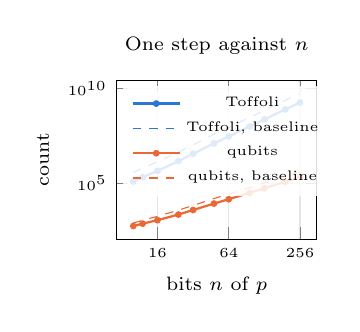
\begin{tikzpicture}
\begin{axis}[width=0.34\linewidth, height=3.6cm, xmode=log, ymode=log, log basis x=2,
  xlabel={bits $n$ of $p$}, ylabel={count}, title={One step against $n$},
  xtick={16,64,256}, xticklabels={16,64,256}, legend pos=north west]
\addplot[cblue, thick, mark=*, mark size=0.8pt] coordinates {(10,120716) (12,203544) (16,441248) (24,1442192) (32,3592352) (48,12552544) (64,29232784) (96,98595488) (128,233652144) (192,785777392) (256,1833327328)};
\addlegendentry{Toffoli}
\addplot[cblue, dashed] coordinates {(10,364970) (12,616882) (16,1338178) (24,4295138) (32,10589570) (48,38598082) (64,88252546) (96,295873666) (128,704262146) (192,2363111426) (256,5459092226)};
\addlegendentry{Toffoli, baseline}
\addplot[corange, thick, mark=*, mark size=0.8pt] coordinates {(10,537) (12,713) (16,1089) (24,2153) (32,3761) (48,8225) (64,13969) (96,30449) (128,53265) (192,117521) (256,204049)};
\addlegendentry{qubits}
\addplot[corange, dashed] coordinates {(10,770) (12,1066) (16,1738) (24,3658) (32,6538) (48,15178) (64,26122) (96,57994) (128,102922) (192,229642) (256,400394)};
\addlegendentry{qubits, baseline}
\end{axis}
\end{tikzpicture}\hfill
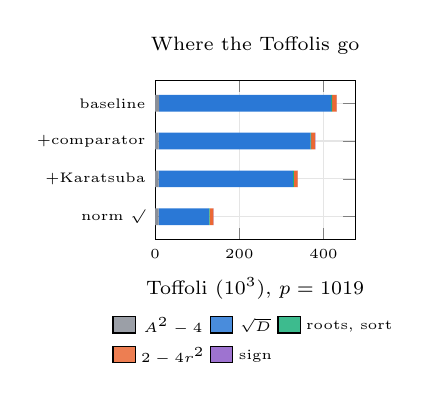
\begin{tikzpicture}
\begin{axis}[width=0.34\linewidth, height=3.6cm, xbar stacked, bar width=6pt,
  xmin=0, xlabel={Toffoli ($10^3$), $p=1019$}, title={Where the Toffolis go},
  ytick={1,2,3,4}, yticklabels={norm $\surd$, +Karatsuba, +comparator, baseline},
  ymin=0.4, ymax=4.6, legend columns=3,
  legend style={at={(0.5,-0.42)}, anchor=north}]
\addplot[fill=cgray, draw=none] coordinates {(8.356,1) (8.356,2) (8.356,3) (9.556,4)};
\addlegendentry{$A^2-4$}
\addplot[fill=cblue, draw=none] coordinates {(119.216,1) (319.142,2) (360.486,3) (408.630,4)};
\addlegendentry{$\sqrt{D}$}
\addplot[fill=caqua, draw=none] coordinates {(1.998,1) (1.998,2) (1.998,3) (2.526,4)};
\addlegendentry{roots, sort}
\addplot[fill=corange, draw=none] coordinates {(9.052,1) (9.052,2) (9.052,3) (10.348,4)};
\addlegendentry{$2-4r^2$}
\addplot[fill=cpurple, draw=none] coordinates {(0.614,1) (0.614,2) (0.614,3) (0.854,4)};
\addlegendentry{sign}
\end{axis}
\end{tikzpicture}\hfill
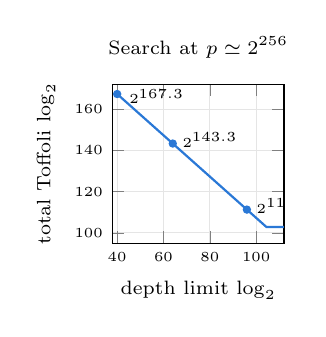
\begin{tikzpicture}
\begin{axis}[width=0.31\linewidth, height=3.6cm, xmin=38, xmax=112, ymin=95, ymax=172,
  xlabel={depth limit $\log_2$}, ylabel={total Toffoli $\log_2$},
  title={Search at $p\simeq2^{256}$}]
\addplot[cblue, thick] coordinates {(40,167.3) (104.4,102.9) (112,102.9)};
\addplot[cblue, only marks, mark=*, mark size=1.3pt] coordinates {(40,167.3) (64,143.3) (96,111.3)};
\node[font=\tiny, anchor=west] at (axis cs:96,113) {$2^{111.3}$};
\node[font=\tiny, anchor=west] at (axis cs:64,145) {$2^{143.3}$};
\node[font=\tiny, anchor=west] at (axis cs:41,166) {$2^{167.3}$};
\end{axis}
\end{tikzpicture}
\caption{Part III. Left: exact cost of one step for primes of $n$ bits (solid: submitted circuit; dashed: baseline). Middle: Toffolis per stage of the step. Right: total cost of the Part II search under a depth limit.}
\label{fig:p3}
\end{figure}

\section{Part IV: Randomly Relabelled (Djinn) Oracle Model}
\footnotesize

Let $V$ be the graph's vertex set, $|V|=N$, and let $\pi:V\to[N]$ be a uniformly random hidden bijection. A vertex name alone is not in general a sufficient routing state: the two legal forward roads depend on the road used to enter the current vertex. Let $e=(u,v)$ denote the directed arrival edge (or use an incoming-port label if parallel edges are present). If the two non-backtracking successors of $e$ are $e_b=(v,w_b)$, define the relabelled successor by
\[
\mathcal N_b(\pi(u),\pi(v))=\pi(w_b),\qquad b\in\{0,1\}.
\]
The coherent neighbour oracle must therefore retain the arrival-edge data, for example
\[
O_{\mathcal N}:|x_{\rm prev},x_{\rm cur},b,z\rangle\mapsto
|x_{\rm prev},x_{\rm cur},b,z\oplus\mathcal N_b(x_{\rm prev},x_{\rm cur})\rangle.
\]
The volunteer predicates depend only on the current name, so their oracle may be written
\[
O_f:|x_{\rm cur},t\rangle\mapsto
|x_{\rm cur},t\oplus f^{\pi}(x_{\rm cur})\rangle.
\]
All input registers are preserved, making these XOR interfaces unitary even when the successor map is not one-to-one. A vertex-only oracle $\mathcal N_b(x)$ describes the original non-backtracking routing rule only if the problem separately defines road labels independently of the incoming road; otherwise the incoming edge/port must be part of the state. The initial state must likewise specify the prescribed starting port or incoming edge.

\textbf{What survives relabelling?} A permutation changes names, not the underlying graph. Degree, adjacency, connectedness, cycles, expansion/spectrum, and the size and location of the marked set as a subset of vertices are preserved. Classical random walks, breadth-first or depth-first exploration with a visited-name table, and collision/cycle detection therefore remain available. If the Clock-Tower density is $\tau=|T_p|/|V|=p^{-1/2+o(1)}$ and the walk is sufficiently mixed, classical random sampling needs $\Theta(1/\tau)=p^{1/2+o(1)}$ marker tests; exhaustive graph exploration costs $O(N)$ neighbour queries and $O(N)$ stored names. Arithmetic operations on $A$, direct $j$-invariant evaluation, Frobenius calculations, and the quaternion/class-group methods are not directly available from opaque names alone.

If the neighbour and marker oracles are genuinely coherent, amplitude amplification over valid directed-edge states or route strings still gives a quadratic search speedup, provided the relevant uniform starting state and inverse oracle are available. Moreover, if a reversible walk on the underlying graph (or a suitable reversible lift) can be accessed coherently, its constant spectral gap can support a MNRS/Szegedy-type quantum-walk search [2,5] with cost
\[
S+O\!\left(\frac{1}{\sqrt{\tau}}
\left(\frac{1}{\sqrt{\delta}}U+C\right)\right),
\]
where $S$ is setup, $U$ is a coherent walk update, $C$ is the coherent marker check, and $\delta$ is the Markov-chain spectral gap. For a constant-gap expander and comparable $U,C$, this is again of order $p^{1/4+o(1)}$ oracle operations. Random naming does not destroy expansion. However, ordinary classical neighbour responses or human volunteers are not coherent oracles: they cannot be queried on a superposition, so Grover and quantum-walk search do not apply to that interface without an efficient reversible implementation of the responses.

\textbf{Searching for both predicates.} If success requires both Clock Tower and ANC, the relevant marked density is
\[
\tau_{\cap}=\frac{|T_p\cap S_{\rm ANC}|}{|V|},
\]
not automatically $\tau_{\rm CT}\tau_{\rm ANC}$. No independence assumption is justified by random relabelling. Conditional densities or an explicit intersection count are needed before assigning a complexity.

\textbf{Lower-bound qualification.} Zalka/BBBV search lower bounds [1,4] give $\Omega(1/\sqrt{\tau})$ quantum marker queries when the marked set is an otherwise unstructured unknown subset and auxiliary oracles reveal no information correlated with it. A random permutation of names alone does not establish that promise: the graph still has exploitable topology, and the true Clock-Tower set is arithmetically correlated with the graph. Therefore the rigorous conclusion is conditional: the $p^{1/4-o(1)}$ lower bound applies to the explicitly unstructured marker-oracle abstraction, not automatically to the full Djinn graph-oracle problem. To claim a lower bound for Part IV, the oracle family must specify whether the marked set is random independently of the graph, whether coherent access is allowed, and what the neighbour oracle reveals.

\begin{thebibliography}{17}\footnotesize\setlength{\itemsep}{0pt}
\bibitem{zalka} C. Zalka, ``Grover's quantum searching algorithm is optimal,'' \emph{Phys. Rev. A} 60 (1999), 2746--2751.
\bibitem{mnrs} F. Magniez, A. Nayak, J. Roland, and M. Santha, ``Search via quantum walk,'' \emph{SIAM J. Comput.} 40(1) (2011), 142--164.
\bibitem{bjs} J.-F. Biasse, D. Jao, and A. Sankar, ``A quantum algorithm for computing isogenies between supersingular elliptic curves,'' in \emph{INDOCRYPT 2014}; related context, but not the assignment's labelled $2$-isogeny algorithm.
\bibitem{bbbv} C. H. Bennett, E. Bernstein, G. Brassard, and U. Vazirani, ``Strengths and weaknesses of quantum computing,'' \emph{SIAM J. Comput.} 26(5) (1997), 1510--1523.
\bibitem{dewolf} R. de Wolf, \emph{Quantum Computing: Lecture Notes}, arXiv:1907.09415, version 6 (27 August 2026). See the chapters on Grover search, quantum walks, and query complexity. \url{https://arxiv.org/abs/1907.09415}.
\bibitem{mit} A. V. Sutherland, \emph{18.783 Elliptic Curves}, MIT OpenCourseWare, Fall 2025. In particular, Lectures 4--6, 12--13, and 16--17 cover isogenies, kernels, torsion, endomorphism algebras, supersingular curves, and complex multiplication. \url{https://ocw.mit.edu/courses/18-783-elliptic-curves-fall-2025/pages/lecture-notes-and-worksheets/}.
\bibitem{florit} E. Florit Zacar\'ias, ``Random walks on supersingular isogeny graphs,'' \emph{Reports@SCM} 6 (2021), 23--34. DOI: 10.2436/20.2002.02.25.
\bibitem{lp} E. Lubetzky and Y. Peres, ``Cutoff on all Ramanujan graphs,'' \emph{Geometric and Functional Analysis} 26(4) (2016), 1190--1216. DOI: 10.1007/s00039-016-0382-7; arXiv:1507.04725.
\bibitem{pizer} A. K. Pizer, ``Ramanujan graphs and Hecke operators,'' \emph{Bulletin of the American Mathematical Society (N.S.)} 23(1) (1990), 127--137. DOI: 10.1090/S0273-0979-1990-15918-X.
\bibitem{mula} M. Mula, N. Murru, and F. Pintore, ``On random sampling of supersingular elliptic curves,'' \emph{Annali di Matematica Pura ed Applicata} 204 (2025), 1293--1335, Theorems 2.13--2.14. DOI: 10.1007/s10231-024-01528-x.
\bibitem{allsolutions} J. van Apeldoorn, S. Gribling, and H. Nieuwboer, ``Basic quantum subroutines: finding multiple marked elements and summing numbers,'' \emph{Quantum} 8 (2024), 1284. DOI: 10.22331/q-2024-03-14-1284.
\bibitem{wesolowski} B. Wesolowski, ``The supersingular isogeny path and endomorphism ring problems are equivalent,'' arXiv:2111.01481 (2021); Cryptology ePrint Archive 2021/919.
\bibitem{pagewes} A. Page and B. Wesolowski, ``The supersingular Endomorphism Ring and One Endomorphism problems are equivalent,'' arXiv:2309.10432 (2023), especially Proposition 8.6 and Theorem 8.7.
\bibitem{delgado} J. L. Delgado, ``The Supersingular Isogeny Problem in Time and Memory $p^{1/3+o(1)}$, Unconditionally,'' arXiv:2609.22018 (18 September 2026).
\bibitem{cdkm} S. A. Cuccaro, T. G. Draper, S. A. Kutin, and D. P. Moulton, ``A new quantum ripple-carry addition circuit,'' arXiv:quant-ph/0410184 (2004).
\bibitem{adj} G. Adj and F. Rodr\'iguez-Henr\'iquez, ``Square root computation over even extension fields,'' \emph{IEEE Trans. Computers} 63(11) (2014), 2829--2841.
\bibitem{bbht} M. Boyer, G. Brassard, P. H{\o}yer, and A. Tapp, ``Tight bounds on quantum searching,'' \emph{Fortschr. Phys.} 46 (1998), 493--505.
\end{thebibliography}
\end{document}
